%%%%%%%%%%%%%%%%%%%%%%%%%%%%%%%%%%%%%%%%%%%%%%
%%
%%    D e s c r i p t i o n    o f     t h e      O b s e r v a t i o n s  : 
%%
%%%%%%%%%%%%%%%%%%%%%%%%%%%%%%%%%%%%%%%%%%%%%%
\smallskip \smallskip
\noindent
We propose to use MIRI MRS to observe four quasars across the full MRS
wavelength range in order to deliver to the community Science Enabling
Products (SEPs) related to the acculmation, reduction and timely
analysis of the MIRI Medium Resolution Spectrometer. Details of our
four quasar targets, including the current state of our extensive
multiwavelength follow-up programs, are given in
Table~\ref{tab:targets}.


\smallskip \smallskip
\noindent
{\bf \underline{Overall Experimental Design}:} 
We have honed in on a specific early release science case that will
engage a broad cross-section of the astronomical community, and
deliver a dataset for MIRI MRS that can be used for e.g. extragalactic
galaxy and AGN studies in Cycle 2.  After discussion with the MIRI
Team (A. Glasse; priv. comm.), we settled on the ideology of picking
out one instrument (MIRI) and one observing mode (MRS) and making sure
we deliver the highest quality data analysis and SEPs here for the
community. Observations with MIRI MRS will also directly answer the
science questions we have posed.

\smallskip \smallskip
\noindent
MIRI MRS is the instrument of choice since no other medium resolution
spectrometer on JWST observes longward of 5μm; going redder than this
is crucial in order to detect PAH features in z > 2 objects. The
desire to immediately gain high signal-to-noise spectra in order to
investigate the physics and chemistry of quasar PAHs, along with
observational overhead concerns, pushes us to observe each object for
3.6 hours, for a total program Charged Time of 22.20 hours.


\begin{table}
\begin{center}
\begin{tabular}{||  l|l|l|l|l ||}
  \hline\hline
  &&&& \\
  Object Name (SDSS)        & J0834+0159         &  J1232+0912          & J2215-0056        & J2323-0100 \\
  &&&& \\
  \hline
  &&&& \\
  Object R.A.                             & 08:34:48.48         & 12:32:41.73           & 22:15:24.00          & 23:23:26.17     \\
  object declination                  & $+$01:59:21.1     & $+$09:12:09.3      & $-$00:56:43.8      & $-$01:00:33.1  \\
  $r$-band AB magnitude         & 21.20$\pm$0.05  & 21.11$\pm$ 0.05  & 22.27$\pm$0.12  & 21.62$\pm$ 0.08 \\  
  WISE W4-band Vega magnitude & 6.88$\pm$0.09  & 6.78 $\pm$0.09   & 7.91$\pm$0.24  & 7.76$\pm$0.22 \\  
  WISE W4-band flux, $F_{\nu}$   & $>$6 mJy             & $>$6 mJy              & 6 mJy                 & $>$6 mJy  \\ 
  $i_{\rm AB}-W3_{\rm AB}$            & 6.0                        & 6.8                        & 6.2                        & 7.2\\

  Redshift $z$        &  2.591                   &  2.381                    &  2.509                  &  2.356 \\  
  &&&& \\
  REW \civ                                 & 209$\pm$6          & 225$\pm$3          &153$\pm$5           &  256$\pm$5\\  
\civ FWHM km s$^{-1}$   & 2863$\pm$65       & 4787$\pm$52       & 4280$\pm$112   & 3989$\pm$62 \\ 
  \oiii\ FWHM erg s$^{-1}$ & 2811                      & 4971                     & 3057                    & 2625 \\ %% From Zam16
  % \oiii FWHM erg s$^{-1}$ & ---                        & 5627                  & 3057                   & 2625 \\ %% From Alexan_the
  &&&& \\
  Spectro-polarimertry       &   $\times$            &  $\surd$                &  $\surd$           & $\times$  \\
  VLA data                          & ?                            &?                             & ?                        & ?  \\ 
  ALMA  Band 6                  & tbc                        & $\surd$                & tbc                     & $\surd$  \\
  {\it HST} Cycle 24           & {\footnotesize ACS/WFC3} &{\footnotesize ACS/WFC3}    & {\footnotesize ACS/WFC3}    & {\footnotesize ACS/WFC3} \\
                                       & {\footnotesize {\bf obtained}}  & {\footnotesize {\it pending}}   & {\footnotesize {\it pending}}  & {\footnotesize {\it pending}} \\
 &&&& \\
JWST target visibility (Start) & 2019-04-01    & 2019-05-08    & 2019-05-22   & 2019-06-07  \\ 
JWST target visibility (End)  & 2019-05-07    & 2019-07-01     & 2019-07-15   & 2019-07-29   \\ 
 &&&& \\
\hline\hline
      \end{tabular}
\caption{
Our four Extremely Red Quasar targets. All four quasars were first
identifired in Ross et al. (2015).  Values of e.g. REWs, FWHMs are
from Zakamska et al. (2016) and Hamann et al. (2017).
}
\label{tab:targets} 
  \end{center}
\end{table}


\section*{MIRI MRS Observing Overview}
We will be utiliSsing the medium-resolution integral field unit (IFU) and spectroscopy mode.  
For our MRS operations we: shall operate over the full wavelength range; 
employ the 4-point dithering pattern, optimized for point sources and using the SLOW  detector read-out mode. For the observations themselves, a wide range of considerations (sample size, desired very high SNR, time available for ERS programs, level of read noise etc.) we converge on:
15 Groups
3 Integrations and 
1 Exposures for a total 
of 12,912 seconds science exposure per object.
{\it Using Smart Accounting, the total Charged Time is 22.20 hours.}


\section*{MIRI Observing Details}
Our observational set-up is:
\begin{itemize}
    \item MIRI MRS.  

    \item Full spectral coverage; thus we will use all three different spectral settings, SHORT (A), MEDIUM (B), and LONG (C).  

    \item Since with the ERQs we are likely to be observing
      either point sources or compact sources, we choose to use the point
      source optimized, ``4-point ALL'' dither pattern (4PTALL
      dither). According to the pre-flight expected relative performance of
      MRS dither patterns (Figure 3,
      https://jwst-docs.stsci.edu/display/JTI/MIRI+MRS+Dithering) this is
      the only MIRI MRS dither patterns that guarantees ``GOOD''
      (i.e. half-integer) sampling throughout the common field of view
      across all four channels.
        We opt for the 4-point ALL dither pattern, point source
        optimized.  As noted in the preparation pages, this provides robust
        performance at all wavelengths and adequate point source separation in
        all channels such that dedicated background observations are not
        required. It is also the only dither where spatial sampling is ``GOOD''
        (i.e. half-integer sampling) throughout the common field of view
        across all four channels.

    \item We are interested in only a single object per point, so no mosaicking is necessary.  

    \item{MIRI Detector Readout mode:: SLOW 
        JWST MIRI's ``Slow mode'' readout pattern offers fewer detector
        artifacts and slightly lower detector noise than the "fast mode",
        making it a good choice for faint source medium-resolution
        spectroscopy where the sky backgrounds are very low. This is 
        exactly what we want for our ERQ observations.}

    \item{Subarray is FULL. This is fixed for MRS.}
\end{itemize}

%
%\begin{wrapfigure}{l}{0.48\textwidth}
%\begin{figure}
  %\begin{center}
%  \includegraphics[height=7.0cm,width=8.5cm]{bias_with_redshift_z3_Sheth01Jing98_20080926.pdf} 
   %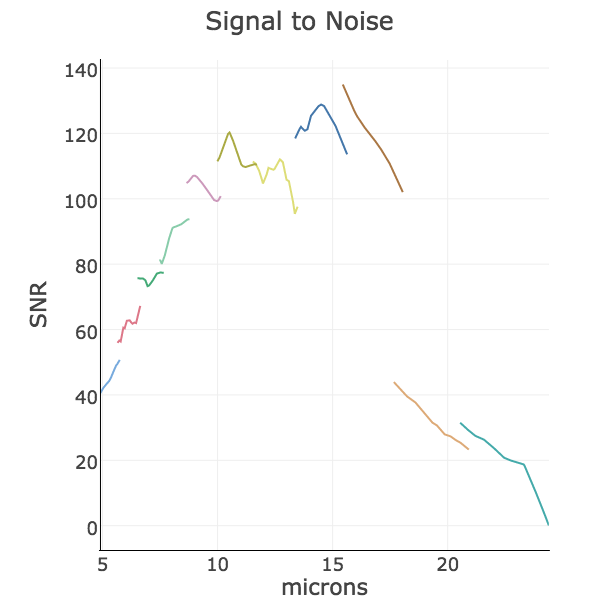
\includegraphics[height=7.0cm,width=7.0cm]{../Figures/current_wavelength_vsSNR.png}
   % \end{center}
  %\caption{The evolution of linear bias, $b$, for SDSS Quasars (Ross et al. 2009).  
   % We find that quasars tend to inhabit haloes of constant mass, $M_{\rm DM} \sim 2 \times 10^{12} M_{\odot}$ 
    %from $z\sim3$ to the present day.} 
  %\label{fig:test-fig}
%\end{figure}
%\end{wrapfigure}

\begin{figure}
  \begin{center}
  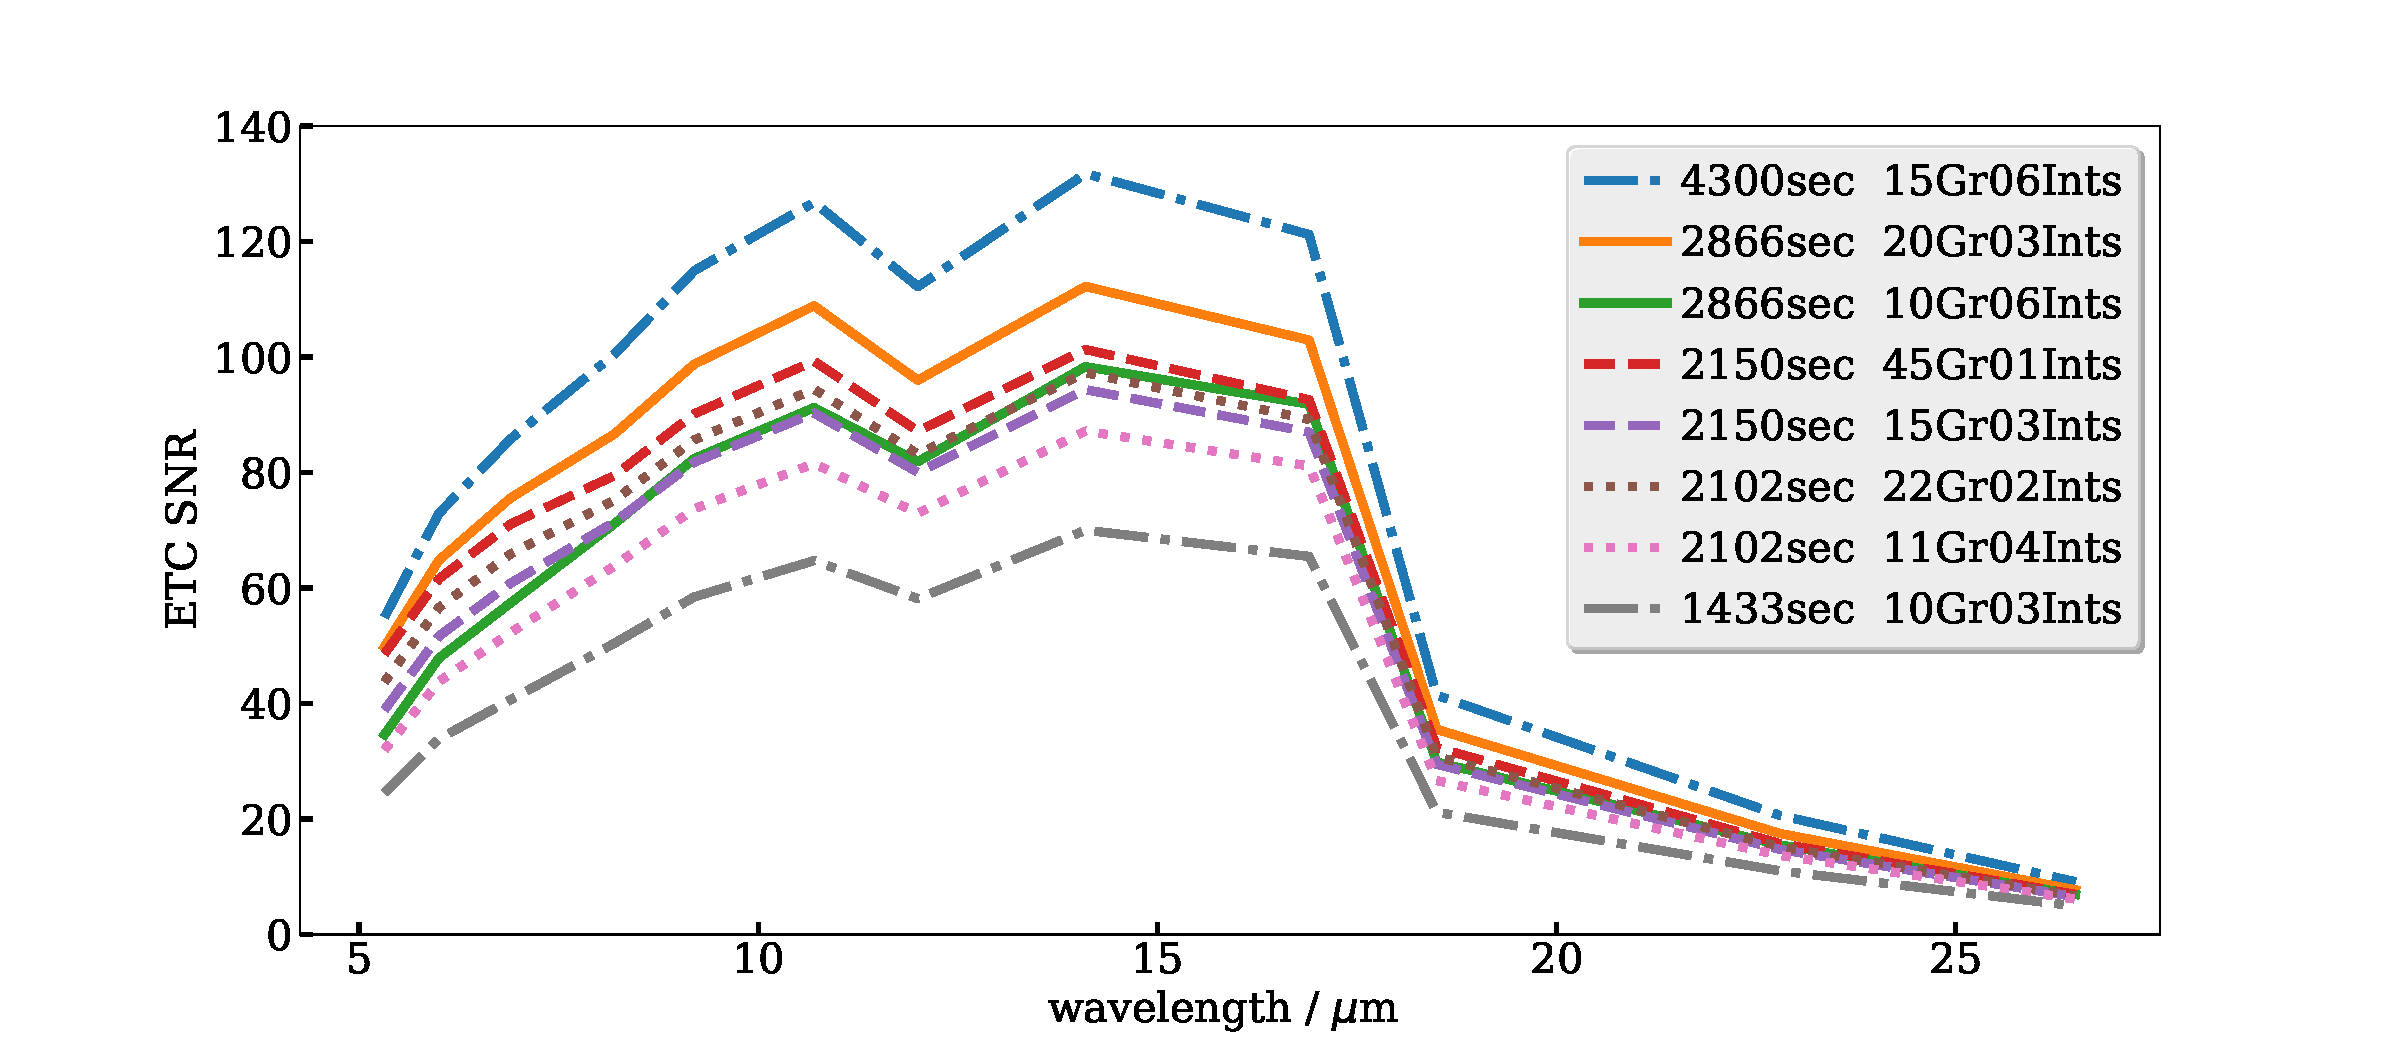
\includegraphics[height=7.0cm,width=16.5cm]{../ETC_calcs/SNR_vs_wavelength_comparisons_full.pdf}
    \end{center}
    \caption{ETC calculations of MIRI SNR values for a range of NGroup
      sizes, Integrations and the associated Science exposure time (per
      Wavelength disperser). }
    \label{fig:test-fig}
  \end{figure}

\smallskip \smallskip 
\noindent
We take the ``core ERQ'' SED that is given in Hamann et al. (2017) and
is fully representative of the ERQ population at large.  The file
(found on the GitHub) of {\tt core\_ERQ\_SED\_notLog.dat} is used
here.  We normalize this SED at a wavelength of 23$\mu$m to a source
flux density of 5mJy, again very representative of the WISE
W3/4-detected ERQ population given in Ross et al and Hamann et al.

\smallskip \smallskip 
\noindent
At this stage we {\it do not} include any emission (or absorption)
lines since...  In the ETC we assume the Shape of the source is Point.
Other notes, using the ETC, include having: Medium Backgrounds; `IFU
Nod In Scene'; Aperture location Centered on source; Aperture radius
of 0.3''; Nod position in scene of $X=Y=0.5''$.  Our JWST ETC Workbook
has \href{https://jwst.etc.stsci.edu/workbook.html?wb_id=7474}{{\tt wb
ID 7474}}.

\iffalse
\begin{table}
\begin{center}
\begin{tabular}{|| l | r | r | r ||}
  \hline\hline
  &&& \\
  Instrument 	& 	Wavelength  & Science          & \multirow{ 2}{*}{SNR} \\
  Setup	        &    	       of Slice  & exp time / s  &        \\
  &&& \\
  \hline
  &&& \\
 Ch1 SHORT & 5.32  &  4778.00 & 44.67 \\
 Ch2 SHORT & 8.20  &  4778.00 & 91.53 \\
 Ch3 SHORT & 12.00  &  4778.00 & 105.07 \\
 Ch4 SHORT & 18.50 &  4778.00 & 38.37 \\
 Ch1 MEDIUM & 6.00  &  4778.00 & 61.69 \\
 Ch2 MEDIUM & 9.20  &  4778.00 & 105.94 \\
 Ch3 MEDIUM & 14.10  &  4778.00 & 125.79 \\
 Ch4 MEDIUM & 22.80  &  4778.00 & 19.84 \\
 Ch1 LONG & 6.90  &  4778.00 & 74.03 \\
 Ch2 LONG & 10.70  &  4778.00 & 117.20 \\
 Ch3 LONG & 16.90  &  4778.00 & 117.22 \\
 Ch4 LONG & 26.50  &  4778.00 & $^{a}$0 \\
  &&& \\
  \hline\hline
\end{tabular}
\caption{Summary of our MRS Instrument Setup, 
  operating wavelengths of the slices and exposure 
  times and SNR. 
  %% 
  % No wavelength overlap between source_spectra [0.42, 23.32] and instrument [23.95, 28.45].
}
\label{tab:ETC_calcs} 
\end{center}
\end{table}
\fi

\subsection*{MIRI MRS Target Acquisition}
%        https://jwst-docs.stsci.edu/display/JTI/MIRI+MRS+Target+Acquisition
Observations with the MIRI MRS IFU may often require a target
acquisition (TA) procedure, especially at the shortest
wavelengths. The required pointing precision for the MIRI MRS is 90
mas (1$\sigma$ radial), which is approximately the half width of a
slice at the shortest wavelength. This required accuracy limits the
spacecraft move between the TA region in the imager and the center of
the IFU to <50" (Sivaramakrishnan et al. 2006).  The TA may be
achieved with the FND, F560W, F1000W and F1500W on either the target
or a suitable offset that is <50". The TA centroiding procedure loses
accuracy if the pixels are saturated so a brightness limit (Table 1)
must be considered for the target.
        % https://jwst-docs.stsci.edu/display/JTI/MIRI+MRS+Dithering

\section*{APT, Overheads and Smart Accounting.}
All the above details in are out APT. 
Visit Planner was loaded and Smart Accounting run. 
Our full proposal comes in at 20.32 hours of charged time. 